\documentclass[a4paper]{article}

\usepackage[english]{babel}
\usepackage[utf8]{inputenc}
\usepackage{amsmath}
\usepackage{graphicx}
\usepackage[colorinlistoftodos]{todonotes}
\usepackage{caption}
\usepackage{subcaption}
\usepackage{here}

\title{Computational Photography}

\author{Mich\`ele Wyss, 10-104-123}

\date{\today}

\begin{document}
\maketitle

\section*{How to use the tool}
Start the code (it's organized in a cell). An image will pop up and you can mark a foreground region using the mouse. As soon as you're done, use the keyboard to indicate whether you want to mark some more foreground regions (1) or move on to marking background regions (0). Then, follow the very same procedure to mark background regions.
\section*{Examples}
See Figures \ref{fig:cow} and \ref{fig:cars}.
\begin{figure}[ht]
	\centering
	%\textbf{Title}\par\medskip
	\begin{subfigure}[h]{0.48\textwidth}
		\centering
		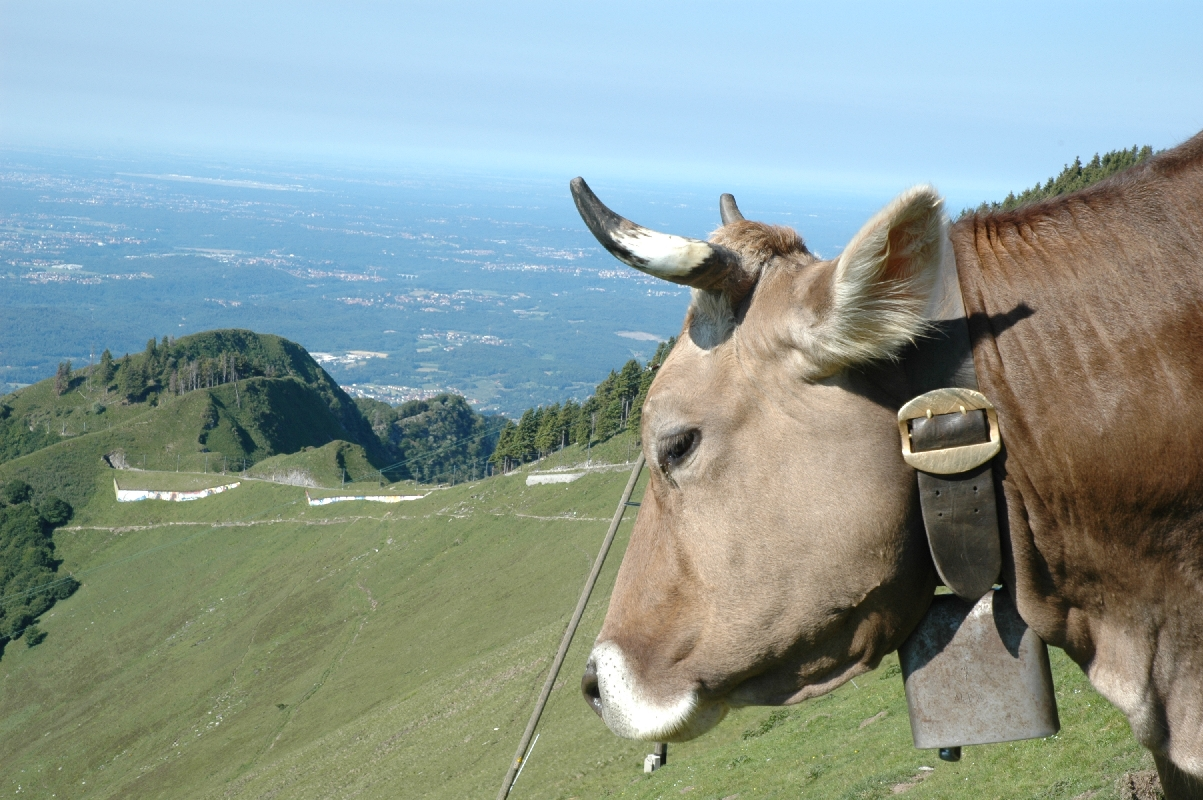
\includegraphics[width=\textwidth]{imgs/cow.jpg}
		\caption*{Input image}
	\end{subfigure}
	
	\vspace{2mm}
	\begin{subfigure}[h]{0.48\textwidth}
	\centering
	
\includegraphics[width=\textwidth]{imgs/bmask.png}
	\caption*{background mask}
	\end{subfigure}
	~
	\begin{subfigure}[h]{0.48\textwidth}
	\centering
	
\includegraphics[width=\textwidth]{imgs/fmask.png}
	\caption*{foreground mask}
	\end{subfigure}
	
	\vspace{2mm}
	\begin{subfigure}[h]{0.48\textwidth}
	\centering
	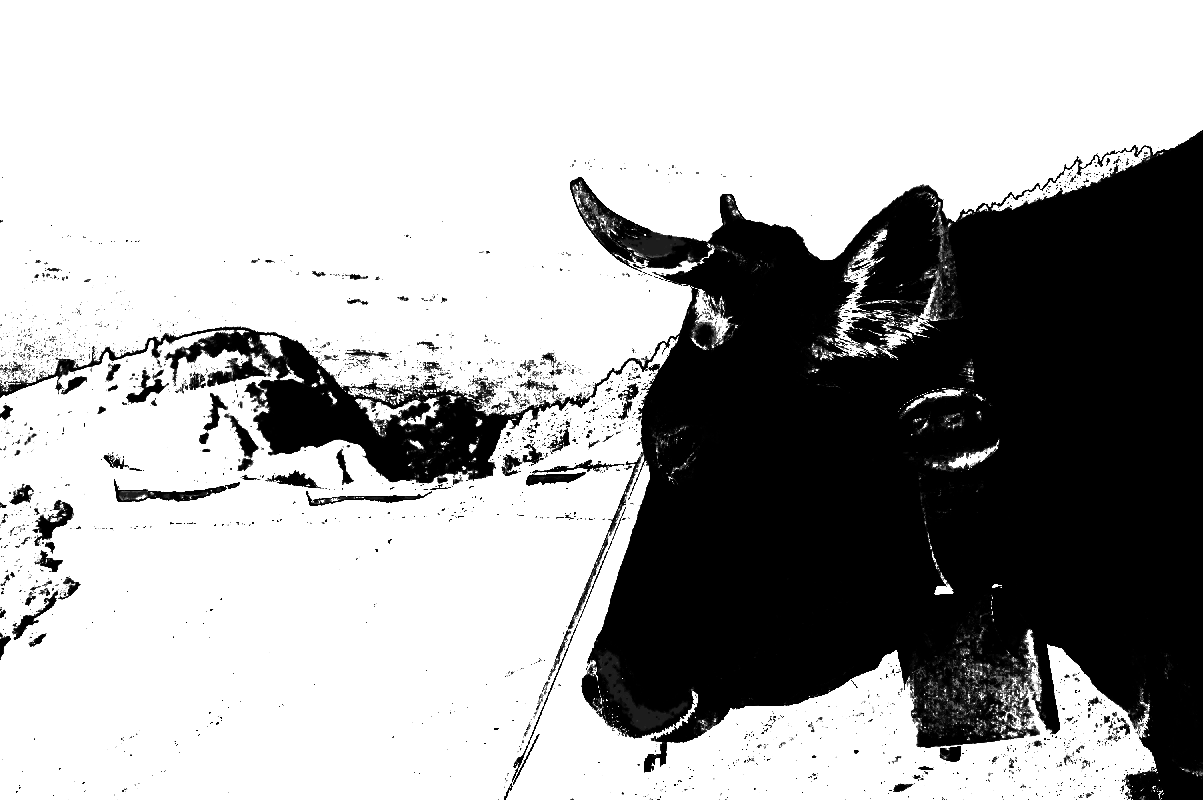
\includegraphics[width=\textwidth]{imgs/backgroundProb.png}
	\caption*{background model probabilities}
	\end{subfigure}
	~
	\begin{subfigure}[h]{0.48\textwidth}
	\centering
	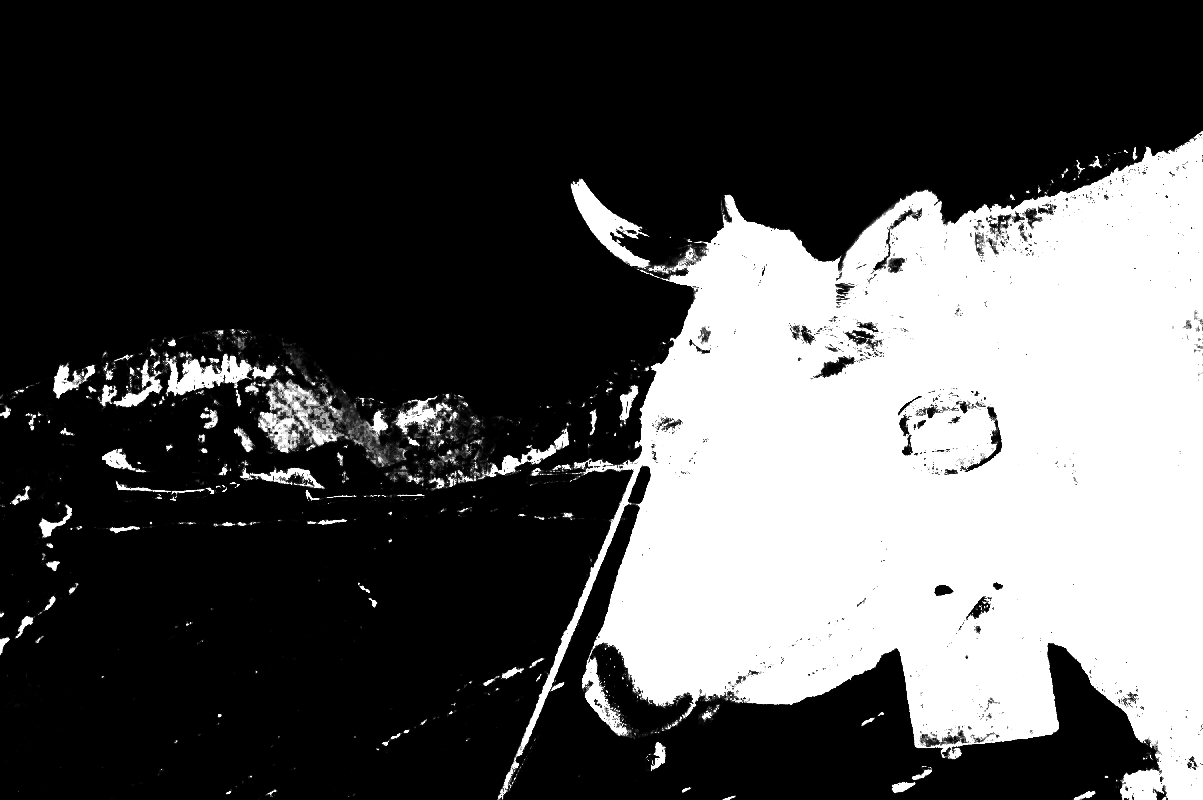
\includegraphics[width=\textwidth]{imgs/foregroundProb.png}
	\caption*{foreground model probabilities}
	\end{subfigure}
		

	
	\vspace{2mm}
	\begin{subfigure}[h]{0.48\textwidth}
	\centering
	
\includegraphics[width=0.48\textwidth]{imgs/backgroundMean1.png}
	
\includegraphics[width=0.48\textwidth]{imgs/backgroundMean2.png}
	\caption*{Average colors of background}
	\end{subfigure}
	~
    	\vspace{2mm}
	\begin{subfigure}[h]{0.48\textwidth}
	\centering
	
\includegraphics[width=0.48\textwidth]{imgs/foregroundMean1.png}
	
\includegraphics[width=0.48\textwidth]{imgs/foregroundMean2.png}
	\caption*{Average colors of foreground}
	\end{subfigure}
\caption{A visualization of the user-generated fore- and background masks and the fitted color models (Gaussian mixture model with 2 components).}
\label{fig:cow}
\end{figure}

\begin{figure}[ht]
	\centering
	%\textbf{Title}\par\medskip
	\begin{subfigure}[h]{0.48\textwidth}
		\centering
		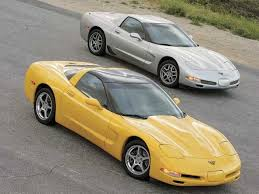
\includegraphics[width=\textwidth]{imgs/fbcars.jpg}
		\caption*{Input image}
	\end{subfigure}
	
	\vspace{2mm}
	\begin{subfigure}[h]{0.48\textwidth}
	\centering
	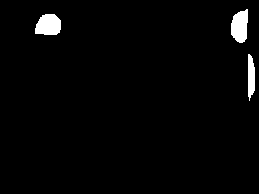
\includegraphics[width=\textwidth]{imgs/bmask_cars.png}
	\caption*{background mask}
	\end{subfigure}
	~
	\begin{subfigure}[h]{0.48\textwidth}
	\centering
	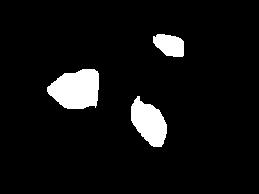
\includegraphics[width=\textwidth]{imgs/fmask_cars.png}
	\caption*{foreground mask}
	\end{subfigure}
	
	\vspace{2mm}
	\begin{subfigure}[h]{0.48\textwidth}
	\centering
	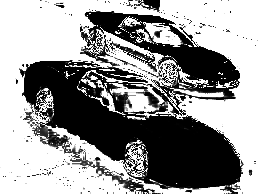
\includegraphics[width=\textwidth]{imgs/backgroundProb_cars.png}
	\caption*{background model probabilities}
	\end{subfigure}
	~
	\begin{subfigure}[h]{0.48\textwidth}
	\centering
	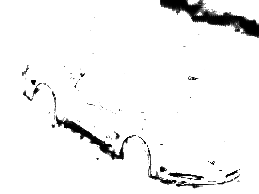
\includegraphics[width=\textwidth]{imgs/foregroundProb_cars.png}
	\caption*{foreground model probabilities}
	\end{subfigure}
		

	
	\vspace{2mm}
	\begin{subfigure}[h]{0.48\textwidth}
	\centering
	
\includegraphics[width=0.32\textwidth]{imgs/backgroundMean1_cars.png}
	
\includegraphics[width=0.32\textwidth]{imgs/backgroundMean2_cars.png}
	
\includegraphics[width=0.32\textwidth]{imgs/backgroundMean3_cars.png}
	\caption*{Average colors of background}
	\end{subfigure}
	~
    	\vspace{2mm}
	\begin{subfigure}[h]{0.48\textwidth}
	\centering
	
\includegraphics[width=0.32\textwidth]{imgs/foregroundMean1_cars.png}
	
\includegraphics[width=0.32\textwidth]{imgs/foregroundMean2_cars.png}
	
\includegraphics[width=0.32\textwidth]{imgs/foregroundMean3_cars.png}
	\caption*{Average colors of foreground}
	\end{subfigure}
\caption{A visualization of the user-generated fore- and background masks and the fitted color models (Gaussian mixture model with 2 components).}
\label{fig:cars}
\end{figure}

\end{document}